\documentclass[linenumbers]{aastex701}
\begin{document}

\title{Quantifying the Impact of TESS Light-Curve Provenance on Machine-Learning Variable-Star Classification}
\author{Jonathan Liang}
\affiliation{Adlai E. Stevenson High School, Lincolnshire, IL, USA}
\email{jonathan.liang1223@gmail.com}

\begin{abstract}
Machine-learning analyses of astronomical time series can depend not only on the classifier and extracted features, but also on how the underlying photometry was produced. This study investigates whether the provenance of Transiting Exoplanet Survey Satellite (TESS) light curves is associated with changes in variable-star classification performance and learned feature importance. We constructed a final TESS light-curve dataset of 7,294 variable stars from the AAVSO International Variable Star Index (VSX), spanning nine broad variable-star classes. The preceding pure-VSX sample contained 8,062 objects and was sampled across 40 requested subtypes using eight right-ascension bins and four approximately equal-area declination bins. A conservative 1\arcsec\ VSX--TESS matching procedure was used to identify suitable TESS observations. For the single closest TIC source within 1\arcsec, a SPOC light curve was used when available, otherwise QLP was used; if neither product was available, photometry was derived from TESSCut full-frame-image cutouts centered on the original VSX position. An initial Random Forest analysis revealed large differences in classification performance among these provenance groups. To separate provenance-associated effects from differences in the underlying stellar populations, matched-star SPOC--TESSCut and QLP--TESSCut experiments were subsequently constructed in which object identity, class labels, train/test assignments, extracted features, and Random Forest configuration were held fixed. The matched experiments show that classification performance and feature-importance rankings remain dependent on light-curve provenance. These results indicate that heterogeneous TESS light-curve products should not automatically be treated as interchangeable inputs to astronomical machine-learning analyses.
\end{abstract}

\keywords{Variable stars --- Time series analysis --- Machine learning --- Random forest --- TESS}

\section{Introduction}
\label{sec:introduction}

\subsection{Variable-Star Classification from Photometric Time Series}
Variable stars exhibit changes in observed brightness over characteristic timescales. Their light curves therefore encode information about the physical processes responsible for the variability as well as the observational properties of the source. As modern surveys produce increasingly large collections of photometric time series, automated classification provides a practical way to organize variable sources into scientifically useful categories.

Machine-learning methods provide one approach to this problem. A light curve can be represented by numerical features describing its flux distribution, time-domain behavior, periodicity, and morphology, after which a supervised classifier learns relationships between those features and previously assigned variable-star labels. Random Forest models are useful in this setting because they can represent nonlinear relationships among features and provide measures of feature importance. In this work, feature importance is not interpreted as direct astrophysical causality; rather, it is used to test whether models trained from different light-curve products rely on the same extracted information.


\subsection{TESS and Heterogeneous Light-Curve Products}
The Transiting Exoplanet Survey Satellite (TESS) provides photometric time-series observations over a large fraction of the sky. TESS observations can be accessed through multiple products and processing pathways. The present study uses three provenance categories: light curves produced by the Science Processing Operations Center (SPOC), light curves produced by the Quick-Look Pipeline (QLP), and light curves derived in this study from full-frame-image cutouts obtained with TESSCut.

These products are related to TESS observations but should not automatically be assumed to be interchangeable representations of an object's variability. Their extraction and processing pathways differ, so measurements associated with the same source can produce different numerical values for variability features. If those features are supplied to a machine-learning classifier, upstream differences can propagate into classification performance and into the model's learned dependence on individual features.


\subsection{The Provenance Problem}
The project initially aimed to construct a Random Forest classifier for variable stars observed by TESS. The input sample was selected from VSX, and each object in the original dataset contributed one usable light curve from SPOC, QLP, or photometry derived from TESSCut. During evaluation of this mixed-provenance dataset, classification performance differed substantially among the three provenance groups. This unexpected result changed the focus of the study from classification alone to a methodological question: \emph{does the provenance of a TESS light curve itself influence downstream machine-learning results?}

The initial observation could not answer this question by itself. Objects with SPOC, QLP, and TESSCut light curves do not form identical stellar samples, and the provenance subsets differ in sample size and class composition. A comparison of their model performance therefore mixes differences in the underlying objects with differences in the light-curve products. The central experimental objective of this work is to separate these factors through matched-star comparisons in which the same objects are analyzed under otherwise identical machine-learning settings.

\subsection{Research Questions and Contributions}
The study is organized around three questions:
\begin{enumerate}
\item Does Random Forest classification performance differ systematically among TESS light-curve provenances?
\item Do models trained from different provenances assign different relative importance to the same set of extracted light-curve features?
\item Do these differences persist when the astrophysical objects, class labels, train/test assignments, feature definitions, and Random Forest configuration are held constant?
\end{enumerate}

To address these questions, we first construct an approximately class-balanced and spatially distributed VSX sample and apply a confidence-first VSX--TESS matching procedure. We then characterize provenance-associated differences in the full dataset and perform two controlled matched-star experiments, SPOC versus TESSCut and QLP versus TESSCut. The purpose is not to introduce a new classification algorithm, but to quantify whether an upstream data-provenance choice changes the behavior of an otherwise fixed machine-learning analysis.

\section{Background and Related Work}
\label{sec:background}

\subsection{Machine Learning for Variable-Star Classification}
Machine-learning classification of variable stars commonly represents each light curve using numerical descriptors and trains a supervised model from objects with known labels. Relevant descriptors can encode the distribution of measured flux, point-to-point variability, periodic structure, and properties of a phase-folded light curve. This feature-based approach is useful for the present study because the same feature definitions can be applied to light curves from different provenances and the resulting models can be compared directly.

Random Forest is the primary classifier used in this work. Logistic Regression was also evaluated as a baseline during model development. The scientific focus, however, is not a comparison of classifier types. Random Forest instead provides a consistent experimental framework in which both predictive performance and learned feature importance can be compared across light-curve provenance. Previous variable-star classification studies establish the broader utility of supervised learning for photometric time series; the present work differs by asking whether changing the upstream TESS light-curve product changes the result obtained from the same downstream analysis.


\subsection{TESS Light-Curve Products}
The three provenance categories enter the analysis through different routes. SPOC and QLP provide pipeline-generated light curves, whereas TESSCut provides image cutouts from which this study derives photometry. Thus, ``provenance'' refers here to the source and processing pathway of the photometric time series supplied to the common feature-extraction and classification pipeline.

\begin{table}[ht]
\centering
\caption{TESS light-curve provenance categories used in this study. Exact processing descriptions will be expanded after verification against the corresponding technical references.}
\label{tab:provenance_overview}
\begin{tabular}{lll}
\hline\hline
Provenance & Input to this study & Light-curve origin \\
\hline
SPOC & Pipeline light curve & SPOC product \\
QLP & Pipeline light curve & QLP product \\
TESSCut & FFI cutout & Photometry derived in this study \\
\hline
\end{tabular}
\end{table}

This difference in processing pathway provides a plausible route by which provenance can influence downstream features. The present paper therefore treats provenance as an experimental variable rather than assuming that all TESS light-curve products are interchangeable.


\subsection{VSX--TESS Cross-Matching and Dataset Construction}
The AAVSO International Variable Star Index provides the source catalog and class labels used to construct the supervised-learning sample. The present study begins from VSX rather than from a pre-existing TESS light-curve catalog. This direction of construction allows the target sample to be selected intentionally across broad variable-star classes, subtypes, and sky position before TESS availability and provenance are determined.

The selected VSX coordinates are associated with TESS sources using the conservative positional-matching procedure described in Section~\ref{sec:dataset}. The method uses a 1\arcsec\ search radius for TIC association and prioritizes a high-confidence positional match. If the matched source has a suitable SPOC or QLP light curve, that product is used; otherwise, TESSCut is used to obtain an image cutout at the original VSX coordinates and photometry is derived from that cutout. Proper-motion checks using SIMBAD are used as an independent validation of the coordinate-based matching strategy.


\subsection{Data Provenance as a Methodological Variable}
A machine-learning model operates on measurements that have already passed through an observational and processing chain. Differences introduced before feature extraction can therefore propagate into the statistical representation seen by the classifier. If provenance changes predictive performance or feature-importance structure, combining heterogeneous products without accounting for their origin can introduce a methodological dependence into the final analysis.

This study tests that dependence empirically. The initial full-dataset analysis establishes whether model behavior is associated with provenance, while the later matched-star experiments test whether the differences persist after major stellar-population confounds are controlled.


\section{Data and Dataset Construction}
\label{sec:dataset}

The dataset was designed for supervised classification while also supporting a later investigation of TESS light-curve provenance. Construction began with labeled variable stars in VSX rather than with objects selected from a particular TESS pipeline. The procedure consisted of four stages: defining a broad variable-star class taxonomy, sampling VSX objects across class and sky position, associating those objects with TESS observations using a conservative matching procedure, and validating the coordinate associations before downstream feature extraction.

\subsection{VSX Source Catalog and Class Taxonomy}
\label{subsec:vsx_taxonomy}

The source population was drawn from VSX. The detailed VSX variability types were consolidated into nine broad variable-star classes used as the supervised-learning labels: \texttt{CEPHEID}, \texttt{CV}, \texttt{DSCT\_SXPHE}, \texttt{ECLIPSING}, \texttt{ELLIPSOIDAL\_ROT}, \texttt{LONG\_PERIOD}, \texttt{RRLYR}, \texttt{XRAY}, and \texttt{YSO}. The classification scheme maps 40 requested VSX subtypes into these nine classes. The XRAY class receives special handling because of its small source population and includes the VSX designations \texttt{HMXB}, \texttt{LMXB}, \texttt{X}, \texttt{XB}, \texttt{XJ}, \texttt{XN}, \texttt{XP}, \texttt{XPR}, and \texttt{XBR}.

The pure-VSX sampling stage applies a target cap of 1000 objects to every class. Eight classes reached that cap, while XRAY contained only 62 available cached records after the expanded XRAY query. The resulting pre-TESS sample therefore contained 8,062 VSX objects.

\begin{table}[ht]
\centering
\caption{Pure-VSX class counts generated before any TIC matching or TESS light-curve acquisition. }
\label{tab:class_taxonomy}
\begin{tabular}{lrr}
\hline\hline
Variable-star class & Target cap & Selected VSX objects \\
\hline
\texttt{CEPHEID} & 1000 & 1000 \\
\texttt{CV} & 1000 & 1000 \\
\texttt{DSCT\_SXPHE} & 1000 & 1000 \\
\texttt{ECLIPSING} & 1000 & 1000 \\
\texttt{ELLIPSOIDAL\_ROT} & 1000 & 1000 \\
\texttt{LONG\_PERIOD} & 1000 & 1000 \\
\texttt{RRLYR} & 1000 & 1000 \\
\texttt{XRAY} & 1000 & 62 \\
\texttt{YSO} & 1000 & 1000 \\
\hline
Total & & 8062 \\
\hline
\end{tabular}
\end{table}


\subsection{Stratified VSX Sampling}
\label{subsec:vsx_sampling}

A simple random draw from VSX could produce a training sample dominated by the most numerous subtypes or concentrated in particular regions of the sky. The pipeline therefore performs sky-balanced sampling before any TESS/TIC matching. The sampling configuration uses eight right-ascension bins and four approximately equal-area declination bins, producing 32 possible RA--Dec sky cells. Validation of the generated pure-VSX sample found all eight RA bins, all four equal-area declination bins, and all 32 RA--Dec cells to be populated across the complete sample.

Within each broad class, the requested count is distributed across the VSX subtypes assigned to that class. Separate VSX web-service queries are issued for subtype--sky-cell combinations, and the returned records are filtered to the relevant logical sky cell. The final class-level selection is then distributed as evenly as practical across populated sky cells until the requested class cap is reached. This procedure is descriptive rather than an assertion of exact spatial uniformity: rare subtypes and intrinsically sparse sky regions can remain underfilled when VSX does not contain enough available objects.

The declination bins are constructed to be approximately equal in sky area rather than equal in angular width. This avoids over-representing high-declination regions merely because lines of right ascension converge toward the celestial poles. After sampling, we evaluated class counts, subtype counts, right-ascension-bin counts, equal-area declination-bin counts, and the two-dimensional RA--Dec cell distribution.


\begin{figure*}[ht]
\centering
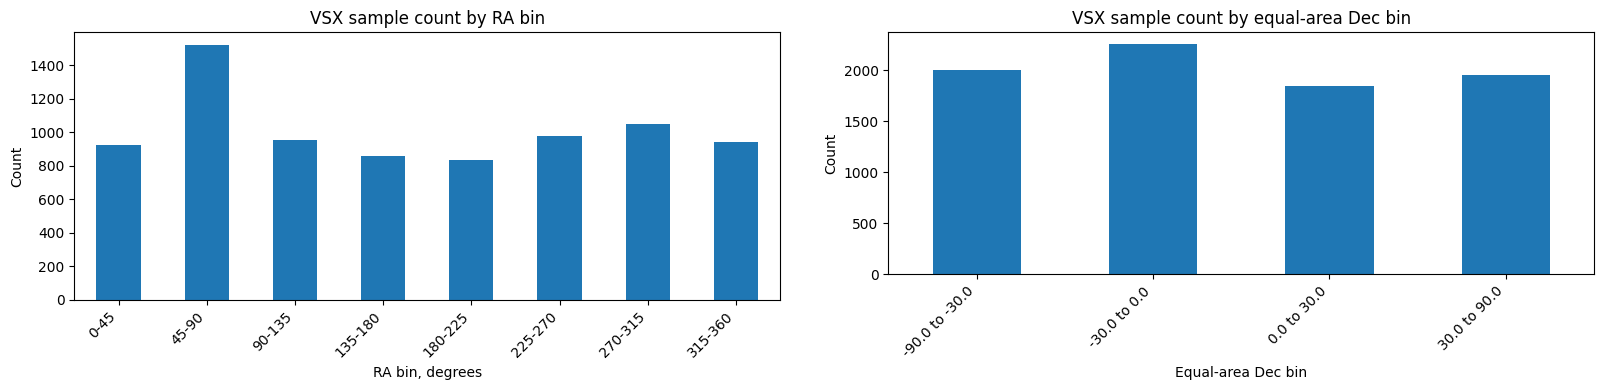
\includegraphics[width=\textwidth]{vsx_sky_sampling_ra_dec.png}
\caption{Sky-distribution diagnostics for the pure-VSX sample before TESS matching. The left panel shows counts in the eight uniform right-ascension bins, and the right panel shows counts in the four approximately equal-area declination bins. All eight RA bins, all four declination bins, and all 32 RA--Dec cells are populated in the 8,062-object pure-VSX sample.}
\label{fig:vsx_sky_sampling}
\end{figure*}

The resulting pure-VSX table contained 8,062 objects distributed across nine classes and 40 requested subtypes. Eight classes contained 1000 objects each, while the XRAY class contained 62. This pre-TESS sampling stage is distinct from the final TESS light-curve dataset, which is smaller after the subsequent matching, acquisition, and cleanup stages.

\subsection{Confidence-First VSX--TESS Matching}
\label{subsec:crossmatch}

For each selected VSX object, the pipeline queries the TESS Input Catalog (TIC) within a radius of 1.0\arcsec. The VSX--TIC angular separation is then recomputed locally from the returned coordinates, and any remotely returned source whose recomputed separation exceeds 1.0\arcsec\ is discarded. Only the single closest surviving TIC candidate is retained; more distant TIC candidates are not examined after that source has been selected.

Light-curve provenance is then assigned using a fixed confidence-first order. For the retained TIC, a SPOC product is used when available. If no SPOC product is available, a QLP product is used when available. If the retained TIC has neither SPOC nor QLP data, the pipeline does not broaden the positional search or inspect another TIC candidate. Instead, it falls back to TESSCut centered directly on the original VSX right ascension and declination.

Conceptually, the procedure is
\begin{equation}
\mathrm{VSX\ position}
\rightarrow
\mathrm{closest\ TIC\ within\ }1\arcsec
\rightarrow
\left\{
\begin{array}{ll}
\mathrm{SPOC}, & \mathrm{if\ available},\\
\mathrm{QLP}, & \mathrm{otherwise\ if\ available},\\
\mathrm{TESSCut\ at\ VSX\ position}, & \mathrm{otherwise}.
\end{array}
\right.
\end{equation}

This design favors association confidence over aggressive catalog matching. Positional reliability is therefore directly relevant to SPOC and QLP rows, which depend on the selected TIC identity. TESSCut extraction is anchored to the VSX position by construction and is evaluated primarily through acquisition success rather than through VSX--TIC separation.

Each object in the original mixed-provenance dataset contributes one light curve and one provenance label. Multiple representations of the same object are generated only later for the matched-star provenance experiments. In those controlled comparisons, TESSCut photometry is extracted at the same VSX coordinates and restricted to the same recorded TESS sector or sector set as the corresponding SPOC or QLP product.


\subsection{Cross-Match Validation}
\label{subsec:match_validation}

Because an incorrect VSX--TIC association could propagate through every later stage of the analysis, the matching strategy was evaluated independently of the machine-learning results. We evaluated the retained TIC separations for SPOC and QLP objects, checked for duplicate selected TIC identifiers, verified acquisition completeness for TESSCut, and performed an independent SIMBAD proper-motion analysis.

\subsubsection{Positional Separation and Duplicate Associations}
\label{subsubsec:positional_validation}

The final augmented dataset contains 1,875 catalog-product light curves whose provenance depends on a retained TIC identity: 509 SPOC and 1,366 QLP objects. All retained SPOC and QLP associations have recomputed VSX--TIC separations below 1.0\arcsec, and in every case the retained source is recorded as the closest candidate.


\begin{table}[ht]
\centering
\caption{VSX--TIC positional-separation statistics for the catalog-product subsets.}
\label{tab:crossmatch_validation}
\begin{tabular}{lrrrr}
\hline\hline
Provenance & $N$ & Median (\arcsec) & 95th pct. (\arcsec) & Maximum (\arcsec) \\
\hline
SPOC & 509  & 0.0500 & 0.4315 & 0.9805 \\
QLP  & 1366 & 0.0411 & 0.3966 & 0.9768 \\
\hline
\end{tabular}
\tablecomments{All retained associations are within 1\arcsec\ and use the closest surviving TIC candidate. The duplicate-selected-TIC audit found zero duplicated TIC identifiers among the SPOC and QLP rows.}
\end{table}

For QLP, the median VSX--TIC separation is 0.0411\arcsec, the 95th percentile is 0.3966\arcsec, and the maximum is 0.9768\arcsec. For SPOC, the corresponding values are 0.0500\arcsec, 0.4315\arcsec, and 0.9805\arcsec. The duplicate-selected-TIC audit found zero cases in which more than one VSX record ultimately pointed to the same retained TIC among the SPOC and QLP rows.

The remaining 5,419 light curves use TESSCut. For these objects, the extraction is requested at the original VSX coordinates, so VSX--TIC separation is not an extraction-error metric.

\subsubsection{Proper-Motion Validation}
\label{subsubsec:proper_motion}

A second validation considered whether stellar proper motion between the catalog reference epoch and the TESS observation epoch could make a fixed 1\arcsec\ matching radius unreliable. For proper-motion components $\mu_{\alpha *}$ and $\mu_{\delta}$ in milliarcseconds per year and a baseline $\Delta t$ in years from J2000.0, the expected angular displacement is
\begin{equation}
\Delta\theta =
\frac{\sqrt{\mu_{\alpha *}^{2}+\mu_{\delta}^{2}}\,\Delta t}{1000},
\label{eq:proper_motion_displacement}
\end{equation}
where $\Delta\theta$ is in arcseconds.

SIMBAD was queried for proper-motion information as an independent validation. For each object, the latest valid TESS sector recorded in the extraction metadata was used to define a conservative observation epoch, because it gives the longest J2000-to-TESS time baseline for objects observed in multiple sectors. We estimate sector midpoints from the continuous sector sequence and then calculate the expected positional displacement.

Of the 7,294 objects in the final augmented dataset, 6,063 (83.12\%) have a nearest SIMBAD match and 5,545 (76.02\%) have published proper-motion measurements. A TESS observation epoch is available for all 7,294 objects, allowing an expected displacement to be calculated for the 5,545 stars with proper-motion data. The median expected displacement is 0.113\arcsec, and the 95th percentile is 0.660\arcsec. A total of 102 stars exceed 1.0\arcsec, corresponding to 1.839\% of the stars for which a displacement could be calculated. The largest predicted displacement is 12.715\arcsec.


\begin{figure}[ht]
\centering
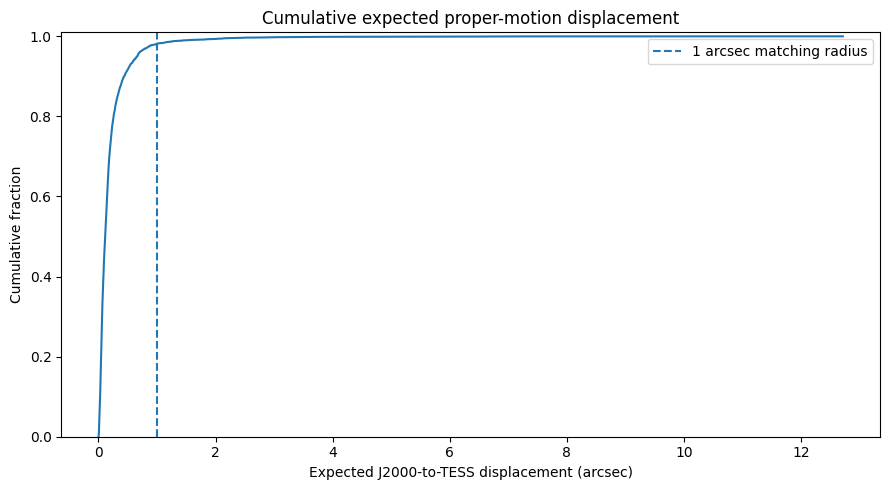
\includegraphics[width=\columnwidth]{proper_motion_cdf.png}
\caption{Cumulative distribution of the expected J2000-to-TESS positional displacement computed from SIMBAD proper motions for the 5,545 objects with usable proper-motion measurements. The dashed vertical line marks the 1\arcsec\ VSX--TIC matching radius.}
\label{fig:proper_motion_cdf}
\end{figure}

These results indicate that the adopted 1\arcsec\ radius remains larger than the predicted J2000-to-TESS proper-motion displacement for the great majority of objects with available measurements. The proper-motion calculation is used as a validation of the population-level matching strategy rather than as an object-by-object correction to the matching algorithm.


\subsection{Final Dataset}
\label{subsec:final_dataset}

The pure-VSX sampling stage produced 8,062 targets before TESS matching. After the subsequent TESS matching, light-curve acquisition, standardization, and cleanup the working dataset contains 7,294 objects. All 7,294 retained objects have an available light curve.

The provenance distribution is 509 SPOC light curves (6.98\%), 1,366 QLP light curves (18.73\%), and 5,419 TESSCut light curves (74.29\%). Thus, SPOC alone covers 6.98\% of the final augmented sample, SPOC or QLP together cover 25.71\%, and the VSX-centered TESSCut fallback brings the acquisition coverage of the retained augmented sample to 100\%.

\begin{table}[ht]
\centering
\caption{Provenance composition of the final TESS light-curve dataset.}
\label{tab:provenance_counts}
\begin{tabular}{lrr}
\hline\hline
Provenance & Number of stars & Fraction \\
\hline
SPOC & 509 & 6.98\% \\
QLP & 1366 & 18.73\% \\
TESSCut & 5419 & 74.29\% \\
\hline
Total & 7294 & 100.00\% \\
\hline
\end{tabular}
\end{table}

The final class totals are also unequal after the TESS acquisition and cleanup stages: 968 CEPHEID, 516 CV, 968 DSCT\_SXPHE, 956 ECLIPSING, 982 ELLIPSOIDAL\_ROT, 963 LONG\_PERIOD, 918 RRLYR, 51 XRAY, and 972 YSO objects. Provenance is not distributed uniformly across these classes. For example, 97.49\% of the final RRLYR sample uses TESSCut, whereas 50.99\% of the LONG\_PERIOD sample uses QLP and 39.22\% of the XRAY sample uses SPOC.

This unequal provenance composition is important for the experimental design. Direct comparisons of the full SPOC, QLP, and TESSCut subsets can reveal provenance-associated patterns, but they cannot by themselves separate provenance from differences in the underlying stellar populations. The later matched-star experiments address this limitation by comparing different products for the same VSX objects while holding the labels, train/test assignments, extracted features, and Random Forest configuration fixed.

\subsection{Dataset-Construction Summary}
\label{subsec:dataset_summary}

The construction procedure was designed to separate two decisions that are often coupled in astronomical machine-learning datasets: which astrophysical objects should be included and which photometric product should represent them. Objects were first selected from VSX according to the variable-star taxonomy and spatial sampling strategy. TESS provenance was then determined through the conservative matching and fallback procedure. This ordering allowed the supervised-learning population to be defined independently of any single TESS pipeline.

At the same time, the 7,294-object augmented TESS dataset remained strongly heterogeneous in provenance. That heterogeneity became scientifically important when the initial classifier showed markedly different performance across SPOC, QLP, and TESSCut objects. Sections that follow describe the common light-curve processing and feature extraction applied before classification and then distinguish the initial unmatched provenance analysis from the matched-star experiments designed to control the underlying stellar population.

% -----------------------------
% End of requested draft.
% Next planned section:
% \section{Light-Curve Processing and Feature Extraction}
% -----------------------------

\end{document}
